Zu einer effizienten Navigation gehört neben geeigneter Techniken auch ein Überblick über die Umgebung, damit sowohl Ziel als auch Weg effektiv gefunden werden können.
Hierfür nutzt der Mensch Karten, um sich eine Vorstellung der Umgebung zu verschaffen (vgl. \textit{wayfinding} \cite{Bowman2001AnDesign}). Dass dies auch - oder sogar vor allem - in virtuellen Umgebungen von Vorteil ist, zeigt die Nutzung von Weltkarten, die inzwischen in einem jedem Computerspiel Standard ist. 

So wurde der positive Effekt von Karten auch in wissenschaftlichen Arbeiten untersucht und dabei Prinzipien gefunden, nach denen Karten in virtuellen Umgebungen designt werden sollen.
Darken et al. \cite{12_Darken1996_WayfindingStrategies} untersuchen in ihrer Arbeit unter anderem Vorgehensweisen der Wegfindung und unterscheiden dabei zwischen \textit{primed search}, also vorbereiteter Suche, und \textit{naive search}, was soviel wie unbefangene oder unvorbereitete Suche bedeutet.
Ersteres meint, dass der Navigierende sein Ziel bereits kennt, zweiteres bedeutet das Gegenteil, Nutzer ihre Ziele also erst finden müssen.
Um die Wegfindung zu vereinfachen schlagen Darken et al. unter anderem vor, die Welt(-karte) in kleinere, einzelne Regionen zu unterteilen und diese durch ein “klares organisatorisches Prinzip” zu strukturieren, da es beinahe unmöglich ist, eine große Welt vollständig abzusuchen. In den unterteilten Regionen sollte der Nutzer stets seine eigene Position sehen können. 
Weiterhin wird die Wegfindung durch Bereitstellen von Richtungsanzeigern und -hinweisen vereinfacht. Solche Hinweise können neben Pfeilen und Wegweisern vor allem einprägsame Orte wie Wahrzeichen und andere Orientierungspunkte sein und sollen bei der Erstellung einer virtuellen Umgebung gegebenenfalls berücksichtigt werden:

\begin{addmargin}[25pt]{0pt} 

\textit{“This has implications for VE designers, who may consider placing the locations they want
people to visit near major topological features, or displaying certain features on maps of
VEs to influence where people are likely to travel.”} \cite{12_Darken1996_WayfindingStrategies}

\end{addmargin}

Bei der Entwicklung ihrer Navigationstechnik, welche im letzten Kapitel vorgestellt wurde, bezogen sich Pierce und Pausch \cite{pierce_representations} auf die Ergebnisse von Darken et al., indem sie ihre Repräsentationen klar hierarchisch organisierten und durch Hochskalieren der wichtigen Orientierungspunkte ihrer Repräsentationen eindeutig erkennbar machen.

Auch Richardson et al. (\cite{Richardson1999}) und Ruddle et al. \cite{Ruddle1999TheEnvironments} untersuchen die Wirkung von Karten und wie sie dazu beitragen eine kognitive Repräsentation der Umgebung zu erzeugen.
Hierbei wird explizit auf den Effekt hingewiesen, den viele beim Lesen eines Stadtplans oder von Strategiespielen (egal, ob auf Brett oder am Computer) selbst schon erlebten: Zwar ist der Mensch in der Lage anhand einer Karte sehr schnell ein genaues kognitives Modell zu erschaffen, dieses ist jedoch beinahe nutzlos, wenn sich die Perspektive dreht.


\begin{figure}[h]
  \centering
  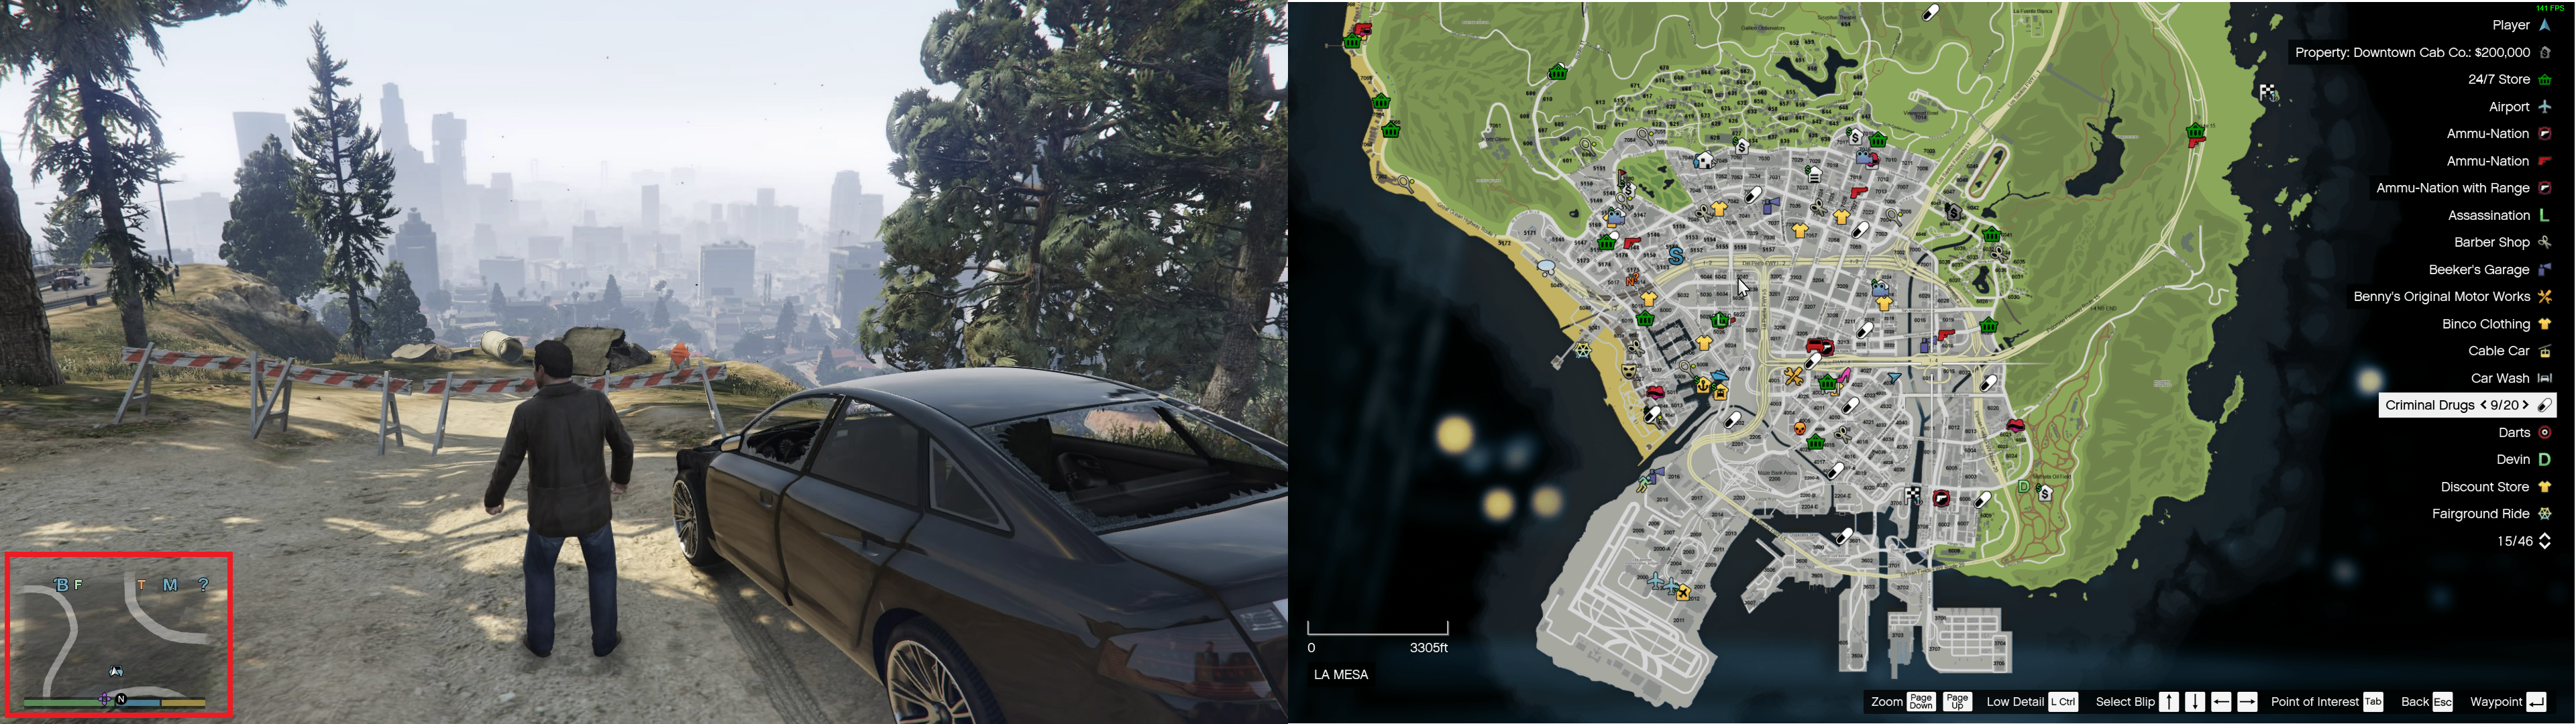
\includegraphics[width=0.8\textwidth]{images/gta.png}
  \caption{In fast allen Computerspielen (wie hier GTA 5), hat sich durchgesetzt, dass dem Spieler zur Orientierung zwei Karten zur Verfügung gestellt werden: Eine Minimap (unten links markiert), die die unmittelbare Umgebung zeigt und stets in Blickrichtung des Spielers ausgerichtet ist, und eine globale Map, die stets nach Norden ausgerichtet ist.}
  \label{fig:todo}
\end{figure}

Dieser Effekt tritt zutage, wenn ein Nutzer die Umgebung zuerst auf einer Karte mit einer Nordrichtung lernt, dann jedoch in einer anderen Ausrichtung in der Umgebung platziert wird. Andersherum ist der Effekt ebenfalls messbar und bekannt. Steht man in einer Stadt und versucht, sich mit der Stadtkarte zu orientieren, dreht man diese häufig so, dass die Oberseite in Richtung der aktuellen Blickrichtung zeigt. Dass das Lernen einer Karte eine orientierungsabhängige, kognitive Repräsentation schafft, wird auch gezeigt, wenn der Mensch versucht sie aus mehreren Perspektiven zu lernen. Dabei ist der kognitive Aufwand allerdings so hoch, dass bei der Abfrage der Raumorientierung Richtungen und Distanzen deutlich schlechter eingeschätzt werden \cite{Richardson1999}.
Mit der Aufteilung der Karte in eine lokale und eine globale Repräsentation schlagen Ruddle et al. \cite{Ruddle1999TheEnvironments} eine Lösung für diese Problematik vor, die heutzutage ebenfalls aus vielen Computerspielen bekannt ist (vgl. Abbildung 5.1). Die lokale Map (in Computerspielen meist “Mini-Map”) ist dabei immer nach dem “Heads Up” Prinzip ausgerichtet, also so wie man es aus dem Beispiel des “Stadtplan-Drehens” kennt, die globale Karte ist stets nach Norden ausgerichtet.

Historisch und praktisch gesehen ist eine Karte für den Menschen zweidimensional, da sie schon seit Jahrtausenden (siehe \cite{meece_2006}) auf Oberflächen gemalt wurden. 
In der virtuellen Realität ist es jedoch ohne Weiteres möglich eine dreidimensionale Repräsentation der Welt zu nutzen, nämlich in Form der bereits erwähnten WIM.
Nutzt man eine solche zur Orientierung, gelten alle bisher genannten Kriterien folglich ebenfalls.
In GulliVR von Krekhov et al. \cite{Krekhov2018GulliVR} wird der Nutzer auf die Größe eines Riesen skaliert und kann somit schnell von A nach B reisen. Die Autoren argumentieren, dass durch diese Form der Reise die Orientierung verbessert wird. Doch man könnte entgegenhalten, dass eine geschrumpfte Welt auch nur eine WIM ist und somit eine andere Form der Karte und nicht das Laufen in dieser Welt die Orientierung verbessert, sondern die Draufsicht, die auch durch eine Karte gegeben wäre.
Dennoch: Durch natürliches Laufen nimmt der Nutzer die “Karte” in einer für ihn ganz natürlichen Art und Weise aus mehreren Orientierungen wahr, sodass der oben genannte Effekt einer statischen Orientierung des kognitiven Abbildes minimiert werden könnte.

Neben den im letzten Kapitel genannten Vorteilen (Interaktion und Navigation) der WIM kann diese also dazu dienen, dass die Nutzer sich eine Vorstellung der Umgebung machen können, ohne dabei an allen Orten der Hauptszene gewesen zu sein. Dabei ist es nützlich, dass in einer WIM, wenn sie denn keine vereinfachte Darstellung ist, stets alle Orientierungspunkte, die man in der echten Welt nutzt, ebenfalls sichtbar sind.
Diese Erkenntnis spricht weiterhin dafür, WIMs zur Navigation zu benutzen und somit eine zweidimensionale Karte der Umgebung, wie sie in vielen Anwendungen genutzt wird, zu ersetzen.
Zu berücksichtigen ist dabei allerdings die Erkenntnis des orientierungsabhängigen, kognitiven Repräsentation. Dabei stoßen nämlich zwei zentrale Eigenschaften aufeinander: Einerseits will man die WIM gerne drehen, damit sie von allen Seiten sichtbar und erreichbar ist. Andererseits kann durch häufiges Drehen der räumliche Lerneffekt gemindert werden. Dies sind beides Gesichtspunkte, die es im Interaktionsdesign zu berücksichtigen gilt.